\documentclass[12pt]{article}
\usepackage{amsmath}
\usepackage{amsthm}
\usepackage{algorithm}
\usepackage{algpseudocode}
\usepackage{amssymb}
\usepackage{graphicx}
\graphicspath{ {assets/} }

\begin{document}

\title{Assignment 5 - Delaunay Triangulation and Voronoi Diagram }
\author{
	Pattarawat Chormai - 0978675 \\
}
\maketitle

\section*{Q2}
Let denote $P$ set of $n$ one euro coins. We first build Voronoi diagram of $P$, $Vor(P)$.
Then, we will move 2 euro coin along each edge of $Vor(P)$ with the constraint that $dist(e_i)$, the distance between a pair
of one euro coins that has $e_i$ as a bisector, is greater than than diameter of 2 euro coin,
$d_{2}$.
We will keep moving until finding a half line edge, which is an exit to the edge of the table,
otherwise we can not move 2 euro coin to the edge of the table without moving one euro coins.

\begin{center}
    \label{figure1}
    \begin{figure}[h]
    \centering
    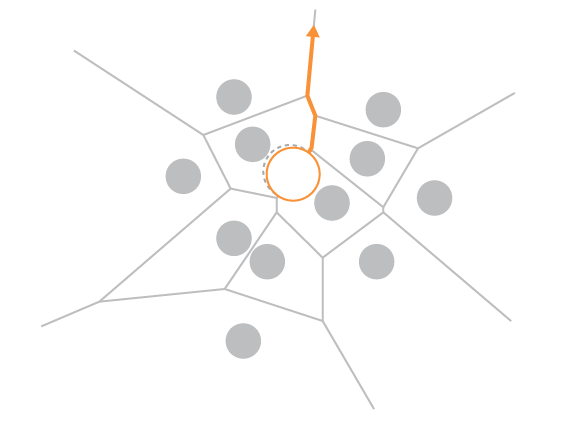
\includegraphics[width=8cm]{voronoi}\\
    \caption{Voronoi diagram as path of moving 2 euro coin } \label{fig:voronoi}
    \end{figure}
\end{center}

The algorithm works as following:
\begin{enumerate}
    \item Build $Vor(P)$
    \item Find $e_o$ that is the closest edge to 2 euro coin.
    \item Perform Depth First Search (DFS) on edges of $Vor(P)$ starting from $e_0$ and examine only $e_i$ whose $dist(e_i) \ge d_2$ \\
       if $e_i$ is a half line, report TRUE
    \item Report FALSE
\end{enumerate}


\subsection*{Correctness}
We know that each edge of $Vor(P)$ is a bisector of a pair of 1 euro coin and the algorithm
always examines the edge that has $dist(e_i)$ big enough. Thus, the path chosen by algorithm
will be always valid. Since DFS is used to traverse edges of $Vor(P)$, if there is a way
from $e_o$ to a half line edge, the algorithm will always find. Therefore, the algorithm
will always report correct result.

\subsection*{Running time}
\begin{enumerate}
    \item Building $Vor(P)$ takes $O(n\log{n})$.
    \item Finding the closest edge $e_0$ takes $O(n)$.
    \item Performing Depth First Search (DFS) takes $O(n)$.
\end{enumerate}

Thus, the algorithm can reports whether there is a way to move the 2 euro coin to the edge
of the table in $O(n\log{n})$.

\end{document}
